\documentclass[11pt,a4paper]{article}                    			% Definierar typ av skrift, textstorlek och pappersformat.
\usepackage{moreverb}                                	% Listor m.m.
\usepackage{lmodern}								% Latin modern font
\usepackage{amsmath}                                	% Matematiska uttryck (American mathematical society).
\usepackage{amssymb}             			% Matematiska uttryck (American mathematical society).
\usepackage{textcomp}                                	% Teckensnitt, symboler m.m.
\usepackage[T1]{fontenc}                            	% Ställer in output.
\usepackage[english]{babel}                            	% Anpassar till engelska (Figurtexter, rubriker m.m.).
\usepackage[utf8]{inputenc}                            % Ställer in input.
\usepackage{graphicx}                                    	% Hanterar bilder m.m.            
\usepackage{subfig}                                    	% Möjliggör flera bilder i en figur.
%\numberwithin{equation}{section}                    % Numrering av ekvationer.
\numberwithin{figure}{section}                         % Numrering av figurer.
\numberwithin{table}{section}                         	% Numrering av tabeller.
\rmfamily                                                 		% Inställning av teckensnitt.
\usepackage{hyperref}								% Enables clickable links in table of contents
\hypersetup{colorlinks,
    		citecolor=black,
   		 	filecolor=black,
    		linkcolor=black,
    		urlcolor=black,
			pdfauthor={David Frisk}}
    		
\usepackage[yyyymmdd,hhmmss]{datetime}	                % Nuvarande datum och tid.
\renewcommand{\dateseparator}{-}

\setlength{\parindent}{0cm}                            % Sätter automatiskt indrag till 0 cm.
\usepackage[labelfont=bf,textfont=it,justification=justified,
singlelinecheck=false]{caption}                      	% Vänsterjusterar caption och gör labeln fet.

\usepackage[
top    = 3cm,
bottom = 3cm,
left   = 3cm,
right  = 3cm]{geometry}				% Ställer in marginaler

\hyphenation{Chalmers} \hyphenation{University} \hyphenation{Technology}

\begin{document}
\begin{center}
{\Large A Chalmers University of Technology\\ Master's thesis template for \LaTeX}\\ [5mm]
David Frisk\\ [5mm]
Updated \today
\end{center}

\section*{Disclaimer}
Please note that this template is not an official template of Chalmers University of Technology (Chalmers). Since Chalmers updated the Master's thesis design recently, most existing Latex (and other) templates are now outdated. I have compiled this template with hope that it can help students in their work until one day when an official Latex template is released.

\tableofcontents

\section{General information}
This template has been constructed based on the following documents and webpages published by Chalmers.

\begin{itemize}
\item Design and publish masters thesis \\ \url{https://student.portal.chalmers.se/en/chalmersstudies/masters-thesis/Pages/design-and-publish-masters-thesis.aspx}

\item Design manual \\ \url{http://www.chalmers.se/insidan/EN/tools/design-manual}

\item Language policy of Chalmers \\\url{http://www.chalmers.se/insidan/EN/tools/language-issues}

\item Regulations for language issues at Chalmers \\ \url{http://www.chalmers.se/insidan/EN/tools/language-issues}

\item Layout of the thesis \\ \url{http://www.chalmers.se/insidan/EN/tools/design-manual/templates/layout-thesis}

\item Vectorized logotypes and emblems \\ \url{http://www.chalmers.se/en/about-chalmers/profile-and-identity}

\end{itemize}


\newpage
\section{Template structure}
Some remarks on the template structure are found below.

\begin{itemize}
\item To create a perspicuous structure of the report source code, each chapter (Abstract, Acknowledgements, Introduction, Methods etc.) and the settings are put in separate .tex files and imported to \texttt{Main.tex} with the \textbackslash\emph{input} macro. The imported files are structured according to  the following schematic.

\begin{figure}[h!]
\centering
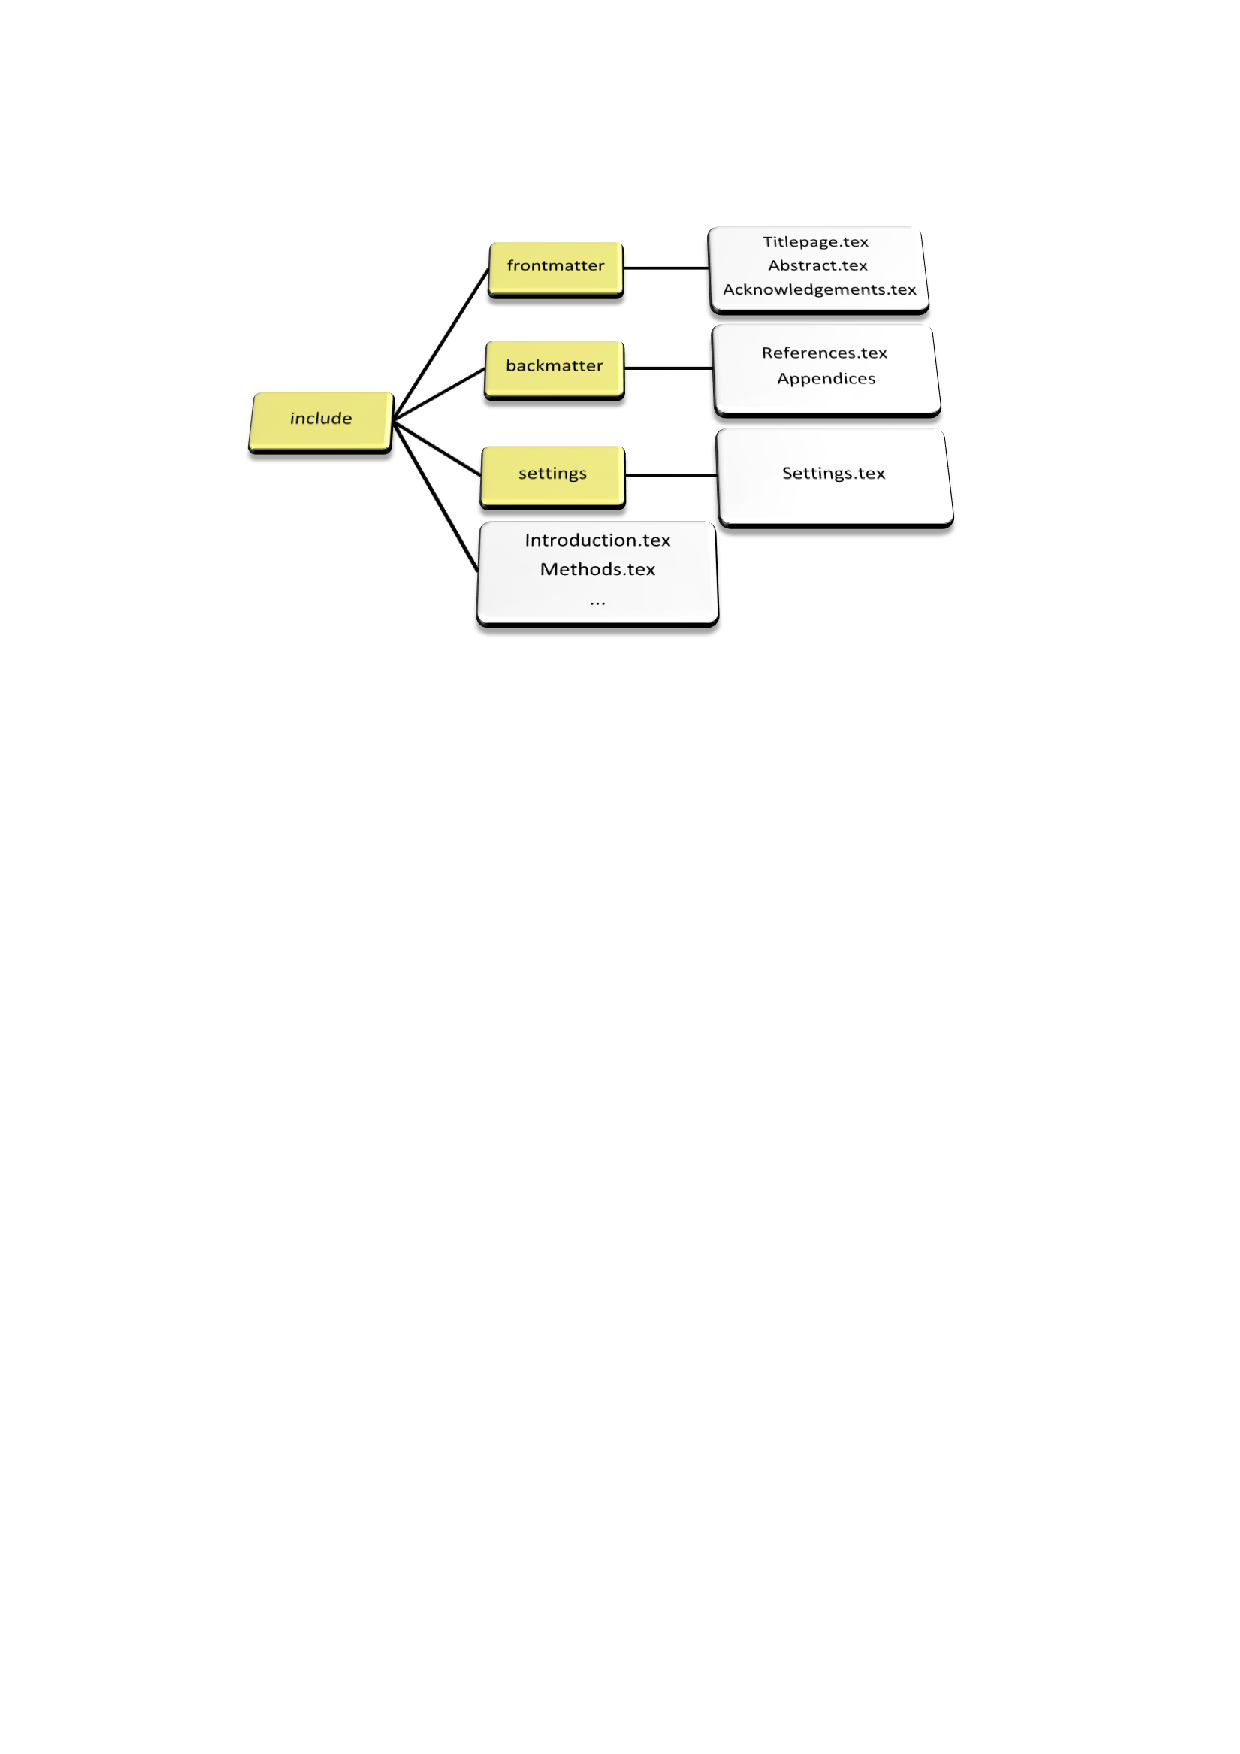
\includegraphics[scale=0.7, trim=3cm 18.5cm 3cm 3.5cm]{Structure.pdf}
\end{figure}

\item In \texttt{Settings.tex}, the required packages are included and some optional settings used to tune the layout of the report are defined. Hence the latter ones can be modified or removed to change the report layout.

\item The template is designed for a two-side layout, meaning that the header and footer are placed in the outer region of the page. This can be modified (for one-side layout) by switching the \emph{design} variable from 2 to 1 above the conditional expression in the \texttt{Settings.tex} file.

\item The Abstract and Acknowledgements are, in the current layout, limited to one page each (which should be enough according to the guidelines). If more pages are required, modifications of the \textbackslash\emph{newpage} positioning are required to make the subsequent chapters start on the right hand side.

\item In the figure/auxiliary folder, the cover page background and Chalmers logotypes are found. There are two versions of these files, one for theses in Swedish (with the logotype text \textsc{chalmers}) and one for theses in English (with the logotype text \textsc{chalmers university of technology}). To change between the two versions (English is default), change between \_eng.pdf and \_swe.pdf where the pictures are imported in the \texttt{Titlepage.tex} file.

\end{itemize}

\newpage
\section{Update history}
\textbf{2015-02-07}\\
Sorted out some warnings regarding underfull hboxes in the frontmatter and included a new object positioning option.

\textbf{2015-02-08}\\
Corrected page numbering error related to the bibliography.

\textbf{2015-02-16}\\
Corrected page numbering errors related to the lists of figures and tables.

\textbf{2016-05-08} \\
Updated year from 2015 to 2016 and fixed minor bugs.


\end{document}